\section{How fast will Raft elect a leader with no split votes?}
\label{leaderelection:nosplit}

\begin{figure}
\centering
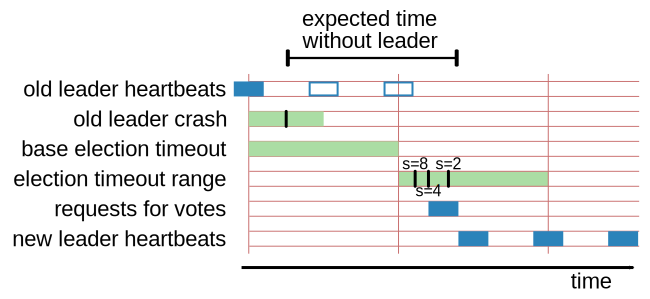
\includegraphics[scale=.55]{leaderelection/timeline}
\vcaption[leader election timeline with no split votes]{
Timeline of a typical election when no split vote occurs.
The first candidate to time out successfully collects votes and
completes the election (other elections may not be so fortunate). The
figure is drawn to scale assuming the election timeouts are chosen from
a range between 10--20 times the cluster's one-way network latency.
\\
The ``old leader heartbeats'' row shows the final heartbeat that the
old leader completes, and when it would have sent its next heartbeats
were it not to crash.
\\
The ``old leader crash'' row shows the interval during which the old
leader crashes. This time is assumed to follow a uniform random
distribution within its heartbeat interval. The vertical line halfway
through the interval is its expected (average) value.
\\
The ``base election timeout'' row shows the interval during which all
the followers await additional heartbeats from the old leader.
\\
The ``election timeout range'' row shows the interval during which the
servers would time out and start elections to replace the old leader.
The vertical lines show expected earliest timeout values for different
numbers of remaining servers (eight, four, and two, respectively).
\\
The ``requests for votes'' row shows when the candidate sends its
RequestVote RPCs to the other servers and receives their votes.
\\
The ``new leader heartbeats'' row shows the new leader sending out
heartbeat RPCs right away after becoming leader, then periodically
thereafter.
}
\label{fig:leaderelection:nosplit:timeline}
\end{figure}

The most common case for leader election in Raft is when no split vote
occurs, and this section analyzes how long it takes to elect a leader
under that assumption. This is expected to be the normal case for Raft
clusters; if the cluster is configured correctly, most normal elections
will not encounter a split vote. The first server to time out will be
able to collect votes from a majority of the cluster and become leader.
The timeline of events is shown in
Figure~\ref{fig:leaderelection:nosplit:timeline}. 

\begin{table}
\centering
\begin{tabular}{ccl}
variable & type & meaning \\
\hline
\noalign{\vskip .75ex}
$s$     & natural & number of available servers \\
$n$     & natural & size of full cluster (including unavailable servers) \\
$c$     & natural & number of servers to time out near each other \\
$l$     & time & constant half round trip network latency (special case of $L$)\\
$L$     & random variable of time & half round trip network latency \\
$W$     & random variable of time & time to write term and vote durably to disk \\
$T_i$   & random variable of time & timeout of server $i$ \\
$M_s$   & random variable of time & earliest timeout of $s$ servers \\
$D_{c,s}$ & random variable of time & difference in timeouts of earliest $c$ of $s$ servers \\
$E_s$   & random variable of time & time to complete an election \\
\end{tabular}
\vcaption[summary of variables]{
Summary of the variables used throughout this chapter to
analyze leader election performance.
Times are normalized to the election timeout range (ranging from 0 to
1).
}
\label{tab:leaderelection:variables}
\end{table}

\begin{figure}
\centering
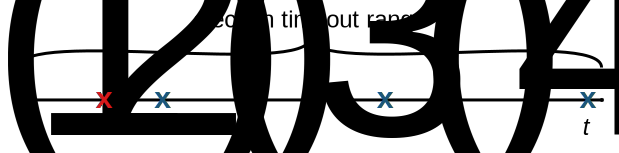
\includegraphics[scale=.5]{leaderelection/earliesttimeoutdiagram}
\vcaption[earliest timeout example]{
What is the smallest random election timeout value chosen by $s$
servers? The diagram shows random election timeouts a five-server
cluster where one server has failed ($s=4$). $t_{(1)}$ is the smallest
timeout value chosen.
}
\label{fig:leaderelection:theory:earliesttimeoutdiagram}
\end{figure}

With no split votes, the time it takes to elect a leader is determined
by how long it takes the first server to time out. The question of when
it will time out is illustrated in
Figure~\ref{fig:leaderelection:theory:earliesttimeoutdiagram}. Each server
waits for a uniform random timeout after the last time it received a
heartbeat. Intuitively, any individual server is expected to time out
halfway through the election timeout range, but with more servers it
becomes more likely that the first server will time out sooner.

We now define the problem more precisely and derive when the first
server times out analytically. The variables defined in this chapter are
summarized in Table~\ref{tab:leaderelection:variables}. Suppose each
server chooses its timeouts randomly from the standard
uniform distribution (in the range $[0,1]$). Let $T_1 \ldots T_s$ be
random variables representing when each of $s$ servers times out. Let $M_s$ be the minimum of
$T_1 \ldots T_s$, a random variable representing the time the first
server times out. Its cumulative distribution function (CDF) defines the
probability that $M_s$ is no greater than a particular time, $t$. This
is equivalent to one minus the probability that all servers times out
after $t$:
\begin{align*}
\Pr(M_s \leq t)
        &= 1 - \Pr(M_s > t) \\
        &= 1 - \prod_{i=1}^s \Pr(T_i > t) \\
        &= 1 - \prod_{i=1}^s (1 - t) \\
        &= 1 - (1-t)^s
\end{align*}
%
For example, consider a cluster with five servers where the prior
leader has failed.
The probability that the earliest of the remaining four servers times out
sometime in the first quarter of the election timeout range is
$\Pr(M_4 \leq \frac{1}{4}) = 1 - (1 - \frac{1}{4})^4 \approx 0.68$.
The CDF is graphed in
Figure~\ref{fig:leaderelection:theory:model:earliesttimeout}
for various values of $s$.

\begin{figure}
\centering
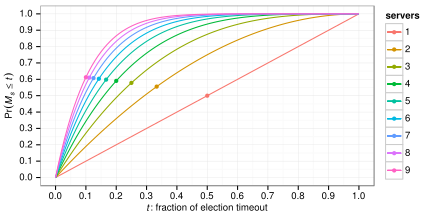
\includegraphics{leaderelection/earliesttimeout}
\vspace{-2ex}
\vcaption[earliest timeout CDF]{
The graph shows the probability that the earliest server times out
before $t$ when different numbers of servers are available. The point on
each line shows the time when the first server is expected to time out
($\Ex[M_s]$).
}
\label{fig:leaderelection:theory:model:earliesttimeout}
\end{figure}

The probability density function (PDF) of $M_s$ is the derivative of the
CDF:
\begin{align*}
 f_{M_s}(t) &= \frac{d}{dt} \Pr(M_s \leq t) \\
        &= \frac{d}{dt} (1-(1-t)^s) \\
        &= -\frac{d}{dt} (1-t)^s \\
        &= s (1-t)^{s-1}
\end{align*}

The expected value (mean) of $M_s$ is calculated from the PDF:
\begin{align*}
 \Ex[M_s] &= \int_0^1 \! t \, f_{M_s}(t) \, dt \\
          &= \int_0^1 \! t (s (1-t)^{s-1}) \, dt \\
          &= \left. \! -\frac{(1-t)^s (s\,t+1)}{s+1} \right|_{t=0}^1 \\
          &= \frac{1}{s+1}
\end{align*}

\noindent
For example, with four available servers, the first timeout is expected
to occur $\dfrac{1}{5}^\textrm{th}$ of the way through the election
timeout range. Fortunately, this very simple expression is a good
estimate of Raft's overall election performance, since elections
complete soon after the first candidate times out when no split vote
occurs.

More precisely, if there is no split vote, the full election requires
a candidate to time out and request votes, once the leader crashes:
\begin{align*}
E_s &= \text{baseline election timeout} + M_s + \text{time to request
votes} - \text{heartbeat adjustment} \\
E_s &= 1 + M_s + 2L + W - U(0,\dfrac{1}{2}) \\
\Ex[E_s] &= 1 + \frac{1}{s+1} + 2\Ex[L] + \Ex[W] - \dfrac{1}{4}
\end{align*}
where election timeouts are chosen from the range $[1,2]$,
$L$ is the network latency, and $W$ is the time to write the votes
persistently to disk.
A uniform random time value from the range $[0, \dfrac{1}{2}]$ is
subtracted, since leaders are expected to crash randomly within their
heartbeat intervals rather than immediately after sending heartbeats.
